%File: formatting-instructions-latex-2023.tex
%release 2023.0
\documentclass[letterpaper]{article} % DO NOT CHANGE THIS
\usepackage{aaai23}  % DO NOT CHANGE THIS
\usepackage{times}  % DO NOT CHANGE THIS
\usepackage{helvet}  % DO NOT CHANGE THIS
\usepackage{courier}  % DO NOT CHANGE THIS
\usepackage[hyphens]{url}  % DO NOT CHANGE THIS
\usepackage{graphicx} % DO NOT CHANGE THIS
\graphicspath{{images/}}

\urlstyle{rm} % DO NOT CHANGE THIS
\def\UrlFont{\rm}  % DO NOT CHANGE THIS
\usepackage{natbib}  % DO NOT CHANGE THIS AND DO NOT ADD ANY OPTIONS TO IT
\usepackage{caption} % DO NOT CHANGE THIS AND DO NOT ADD ANY OPTIONS TO IT
\frenchspacing  % DO NOT CHANGE THIS
\setlength{\pdfpagewidth}{8.5in}  % DO NOT CHANGE THIS
\setlength{\pdfpageheight}{11in}  % DO NOT CHANGE THIS
%
% These are recommended to typeset algorithms but not required. See the subsubsection on algorithms. Remove them if you don't have algorithms in your paper.
\usepackage{algorithm}
\usepackage{algorithmic}
\usepackage{todonotes}

%
% These are are recommended to typeset listings but not required. See the subsubsection on listing. Remove this block if you don't have listings in your paper.
\usepackage{newfloat}
\usepackage{listings}
\DeclareCaptionStyle{ruled}{labelfont=normalfont,labelsep=colon,strut=off} % DO NOT CHANGE THIS
\lstset{%
	basicstyle={\footnotesize\ttfamily},% footnotesize acceptable for monospace
	numbers=left,numberstyle=\footnotesize,xleftmargin=2em,% show line numbers, remove this entire line if you don't want the numbers.
	aboveskip=0pt,belowskip=0pt,%
	showstringspaces=false,tabsize=2,breaklines=true}
\floatstyle{ruled}
\newfloat{listing}{tb}{lst}{}
\floatname{listing}{Listing}
%
% Keep the \pdfinfo as shown here. There's no need
% for you to add the /Title and /Author tags.
\pdfinfo{
/TemplateVersion (2023.1)
}

\setcounter{secnumdepth}{0} %May be changed to 1 or 2 if section numbers are desired.

\title{CS-GY 6953 / ECE-GY 7123 Miniproject}
\author {
    % Authors
    Casey Primel,\textsuperscript{\rm 1}
    Chimnay Tompe, \textsuperscript{\rm 2}
    Saikaran Nakka \textsuperscript{\rm 3}
}
\affiliations {
    % Affiliations
    \textsuperscript{\rm 1} Computer Science\\
    \textsuperscript{\rm 2} Electrical Engineering\\
    \textsuperscript{\rm 3} Computer Engineering\\
    ctp219@nyu.edu, cst9314@nyu.edu, svn9710@nyu.edu
}



\begin{document}

\maketitle

\begin{abstract}
Convolutional neural networks and, most recently, transformer-based models dominate deep learning for computer vision. Models based on these architectures achieve high accuracy often at the expense of computational complexity, with even the tiniest examples rarely having less than 5 million parameters. For our miniproject, we experimented with a newer architecture, ConvMixer, a convolutional network with skip connections that incorporates aspects of transformers and other more recent architectures to outperform similarly sized models despite its relative simplicity. Our model achieves 94.3\% accuracy on CIFAR-10 classification after 100 training epochs while using less than 12\% of our allocated 5 million parameter budget. Our code is available at \url{https://github.com/cprimel/cautious-fiesta}.
\end{abstract}

\section{Introduction}

Depth is a significant factor for the success of artificial neural networks in computer vision tasks, but that significance has often confounded by the difficulties of training such deep networks. One such difficulty is degradation: as layers are added to a deep neural network one would naively expect model accuracy to improve because the model would be able to capture a better feature representation of the data; however, in practice, the opposite was observed. Mathematically, we can understand this in terms of our model $\mathcal{F}$ trying to approximate a true function $f^*$. If a new layer is added such that we move from $\mathcal{F}$ to $\mathcal{F}^\prime$, there is no guarantee that our new model gets us any closer to $f^*$. The only way to make this guarantee is if we can constrain $\mathcal{F}^\prime$ such that $\mathcal{F} \subset \mathcal{F}^\prime$.\footnote{This particular mathematical interpretation of degradation is drawn from \citet{Zhang2021}, specifically Chapter 8.6.1 building on the original explanation of \citet{He2015}.}

\citet{He2015} proposed the introduction of a residual learning framework, often referred to as skip connections, as a means of constraining $\mathcal{F}^\prime$. Rather than each successive layer needing to learn a new mapping $f(\mathbf{x})$, where $\mathbf{x}$ is the output from the previous layer, we deliberately train the new layer towards the identity $f(\mathbf{x})=\mathbf{x}$ by carrying $\mathbf{x}$ forward and have our additional layer learn $g(\mathbf{x}) = 0$, where $f(\mathbf{x})= g(\mathbf{x}) + \mathbf{x}$. In addition, the computational costs of the added complexity is miniscule requiring only an additional addition operation per each residual block. These characteristics have led to skip connections being a common component in modern deep learning architectures, even transformer-based models. 

If skip connections have opened up depth, transformers have turned the focus to the representation of image data. In the context of convolutional neural networks (CNNs) like ResNet, images are represented at the per-pixel level with the hierarchical structure of the image being constructed as one moved deeper into the network via repeated convolutions and pooling operations. Transformers, due to the computational complexity of their self-attention layers, necessitate representing images as multiple patches analogous to tokens in natural language processing \citep{Dosovitskiy2020}. Whereas per-pixel representation in CNNs allows the successive layering of the global structure of an image, patch embeddings encode both the local and global structure of an image for transformer-based models. However, patch embeddings can also be used in combination with other architectures to separate out the work of pulling out the local features and global structures that comprise an image. It's in this vain that \citet{Tolstikhin2021} propose the MLP-Mixer, an architecture based around multi-layer perceptrons which explicitly splits the operations of or per-location (local) and cross-location (global), which they refer to as \textit{channel-mixing} and \textit{token-mixing}, respectively. 

The following report describes our experiments with applying the ConvMixer architecture to the CIFAR-10 dataset \citep{Krizhevsky2009LearningML}. ConvMixer takes the insights of transformer-based models but, unlike MLP-Mixer, achieves channel- and token-mixing through standard convolutional layers withskip connections. Like the MLP-Mixer it is also an isometric architecture, making it somewhat akin to other isometric residual networks as examined by \citet{Sandler2019}. Our final model has 594,186 parameters and achieves 95\% accuracy on CIFAR-10 after 200 training epochs.

\section{Methodology}

The choice of architecture was primarily driven by the goal of maximizing model performance while minimizing the number of parameters. Initial explorations showed that a typical small architecture, e.g., ResNet10, clock in at just under the proscribed limit of 5 million parameters and could achieve well over the required 80\% baseline with standard regularization. In fact, tiny architectures were able of performing just as well if not better on a small dataset like CIFAR-10. For instance, the 3-layer\footnote{\citet{He2015} use the term layer to refer both to the convolution operator and the set of residual blocks that share the same output width. Here we use the latter to distinguish between the typical 4-layer and the simplified 3-layer architecture for CIFAR-10.} ResNet described by \citet{He2015} for use on CIFAR-10 were capable of 91\% and 93\% with only .27 and 1.7 million parameters, respectively. However, most research only treats CIFAR-10 as a secondary objective with models being trained on and primarily benchmarked against the ImageNet or the proprietary JFT-300M dataset. A good example of this is ViT architecture presented by \citet{Dosovitskiy2020} which achieves over 98\% on CIFAR-10 after pre-training at the cost of 86 million parameters.


\subsection{ConvMixer architecture}



\todo{describe architecture}

\todo{add diagram}

Our implementation is drawn directly from \citet{trockman2022patches}, in particular the "more readable" PyTorch implementation presented in Appendix D. 

\subsection{Training setup}

Training and testing were performed via command line scripts. The training script is heavily inspired by \verb|timm| \citep{rw2019timm} the principle differences being that we aimed to only use built-in PyTorch functions where they were available, a simplified model registry structure and the focus on CIFAR-10 dataset. 

Each experiment is defined in a YAML file and fed to the training script. Training checkpoints are saved only if the accuracy of the epoch is better than all previous epochs and the training log with metrics for each epoch are output as a JSON file allowing for post-run analysis. Tests are run on the best checkpoint from training and a log containing the predicted and true labels for all test images is saved to JSON.

All models were trained and tested in Google Colab-hosted Jupyter notebooks running on a GPU instance (running a 16 GB Tesla T4).

\subsection{Experiments}

The results of the CIFAR-10 ablation study performed by \citet{trockman2022patches} with the ConvMixer architecture provided an initial basis for choosing the model parameters and regularization techniques we applied in our experiments. \citet{trockman2022patches} show that increasing kernel sizes result in more parameters with decreasing gains to accuracy while larger patch sizes lead to rapid decreases in accuracy. These empirical results make sense given the small input size. We focused on ConvMixer256/8 alternating between kernel sizes of 5 and 9 and patch sizes of 1 and 2. We also ran an experiment doubling the depth of the network to 16, i.e., ConvMixer256/16, to see exactly how much training behavior changed with increased depth; however, we decided that the increased training time and, thus, our inability to iterate further experiments on the model in a timely fashion, far outweighed any accuracy increases we could squeeze out of it.

Our results differ likely in large part to the fact that we use the PyTorch implementation for nearly all the relevant model components (e.g., optimization algorithms) whereas \citet{trockman2022patches} use those provided in \verb|timm|.

\begin{table}
    \begin{tabular}{|c|c|c|c|c|}
        \hline
        \hline 
        Depth & Kernel size & Patch size & Parameters & Best acc. (\%) \\
        \hline
        8 & 5 & 1 & 591,882 & 94.1 \\
        8 & 5 & 2 & 594,186 & 94.5 \\
        8 & 9 & 1 & 706,570 & ??? \\
        8 & 9 & 2 & 708,874 & 94.3 \\
        16 & 9 & 2 & 1,411,338 & 91.9 \\
        \hline
    \end{tabular}
    \caption{Selection of tiny ConvMixers, all $h=256$ trained for 100 epochs on CIFAR-10.}
\end{table}

\begin{figure}
    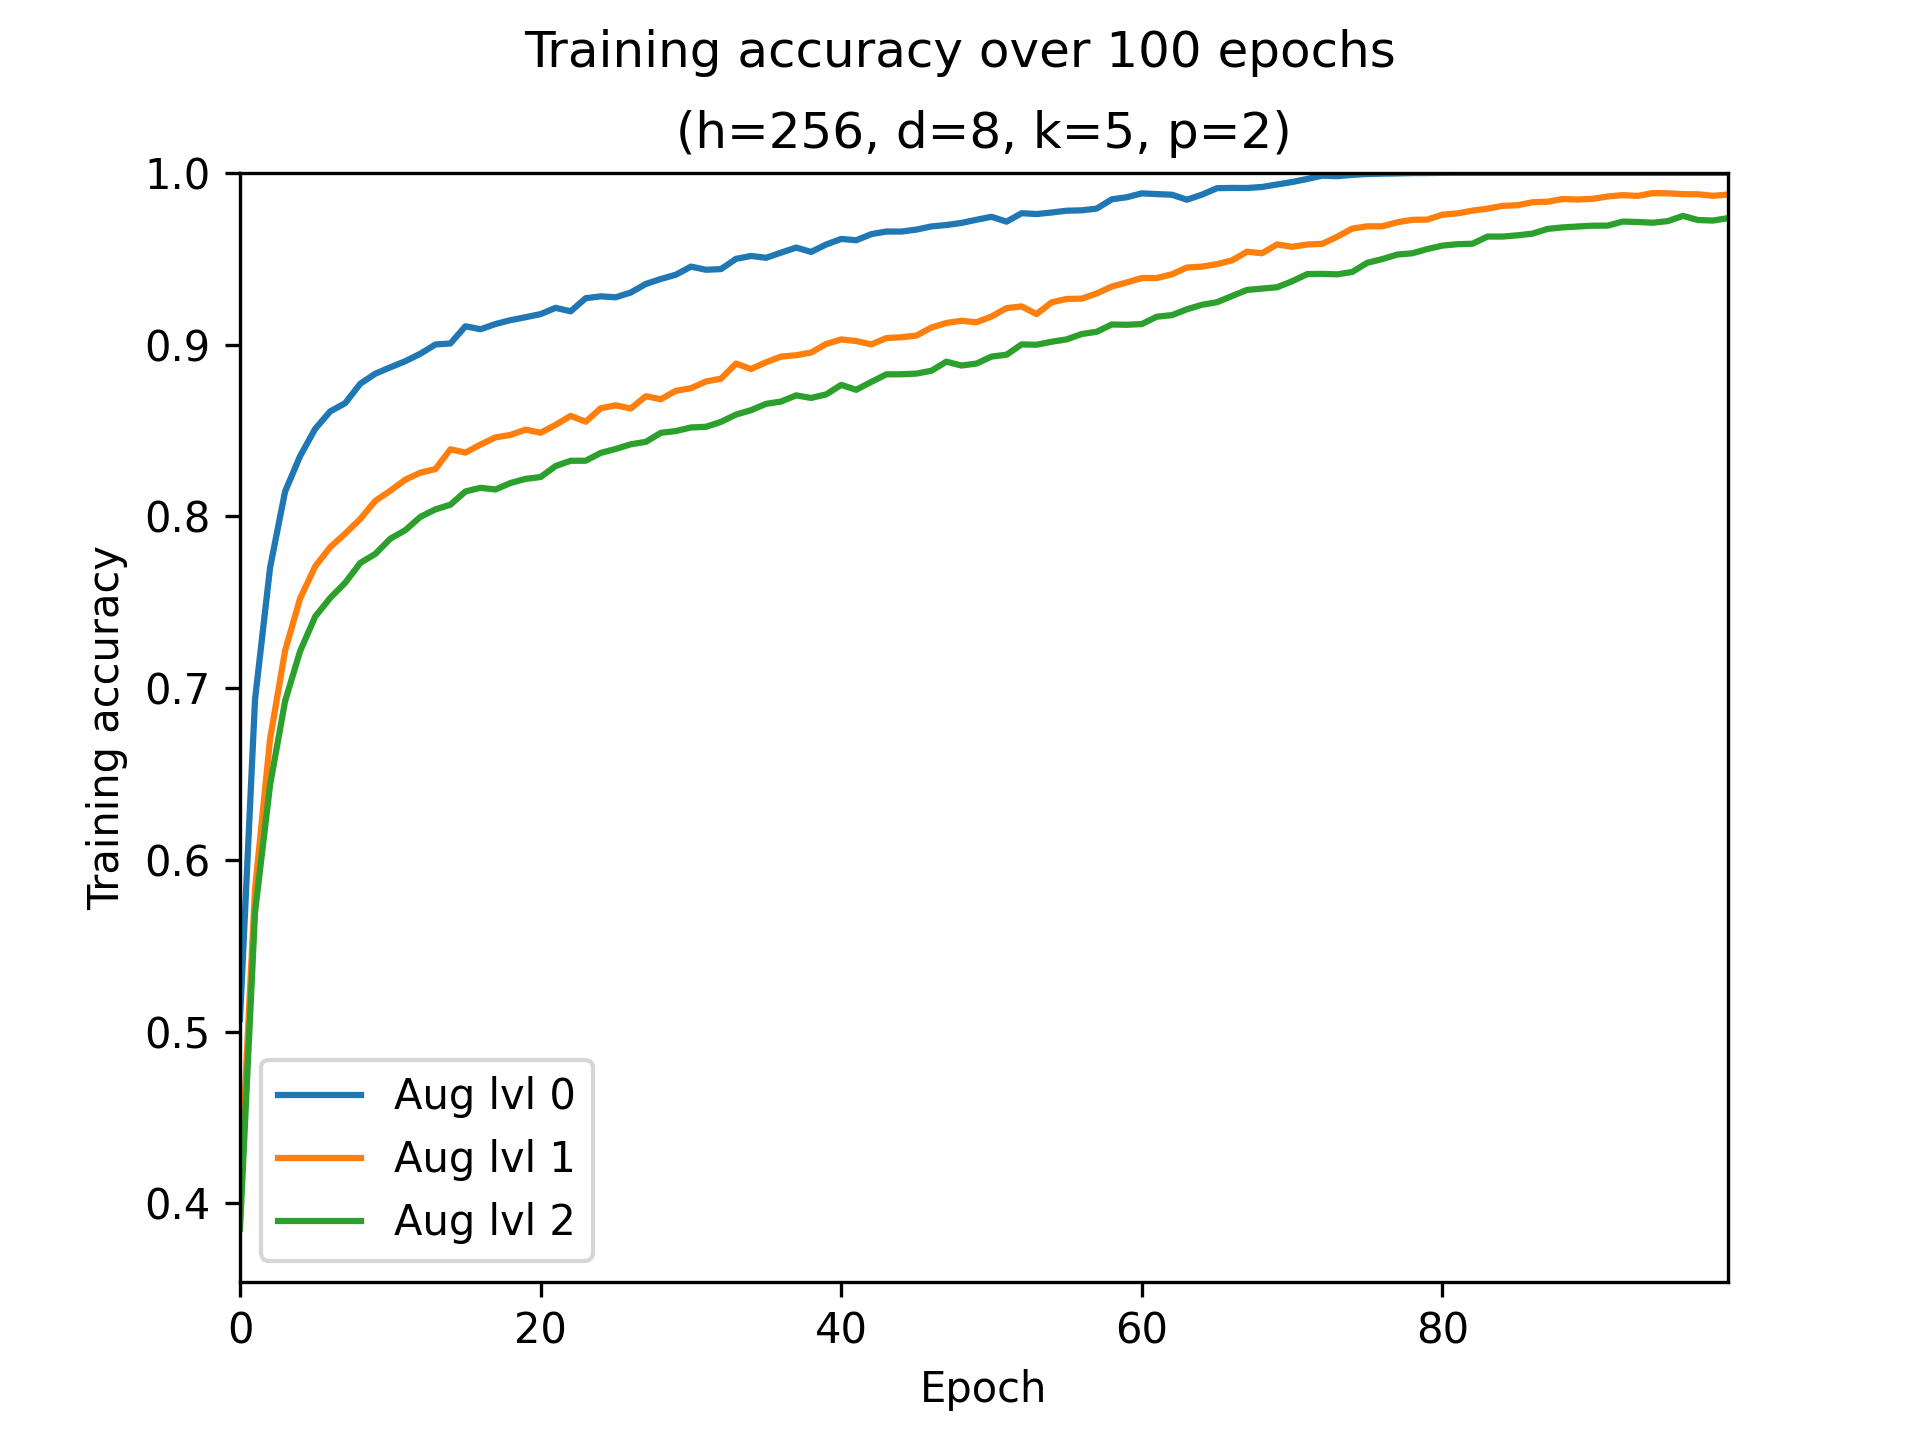
\includegraphics[width=\linewidth]{training_k5p2.png}
    \caption{Comparison of model training metrics for ConvMixer256/8 (kernel size=5, patch size=2) at different augmentation levels.}
  \end{figure}

  \begin{figure}
    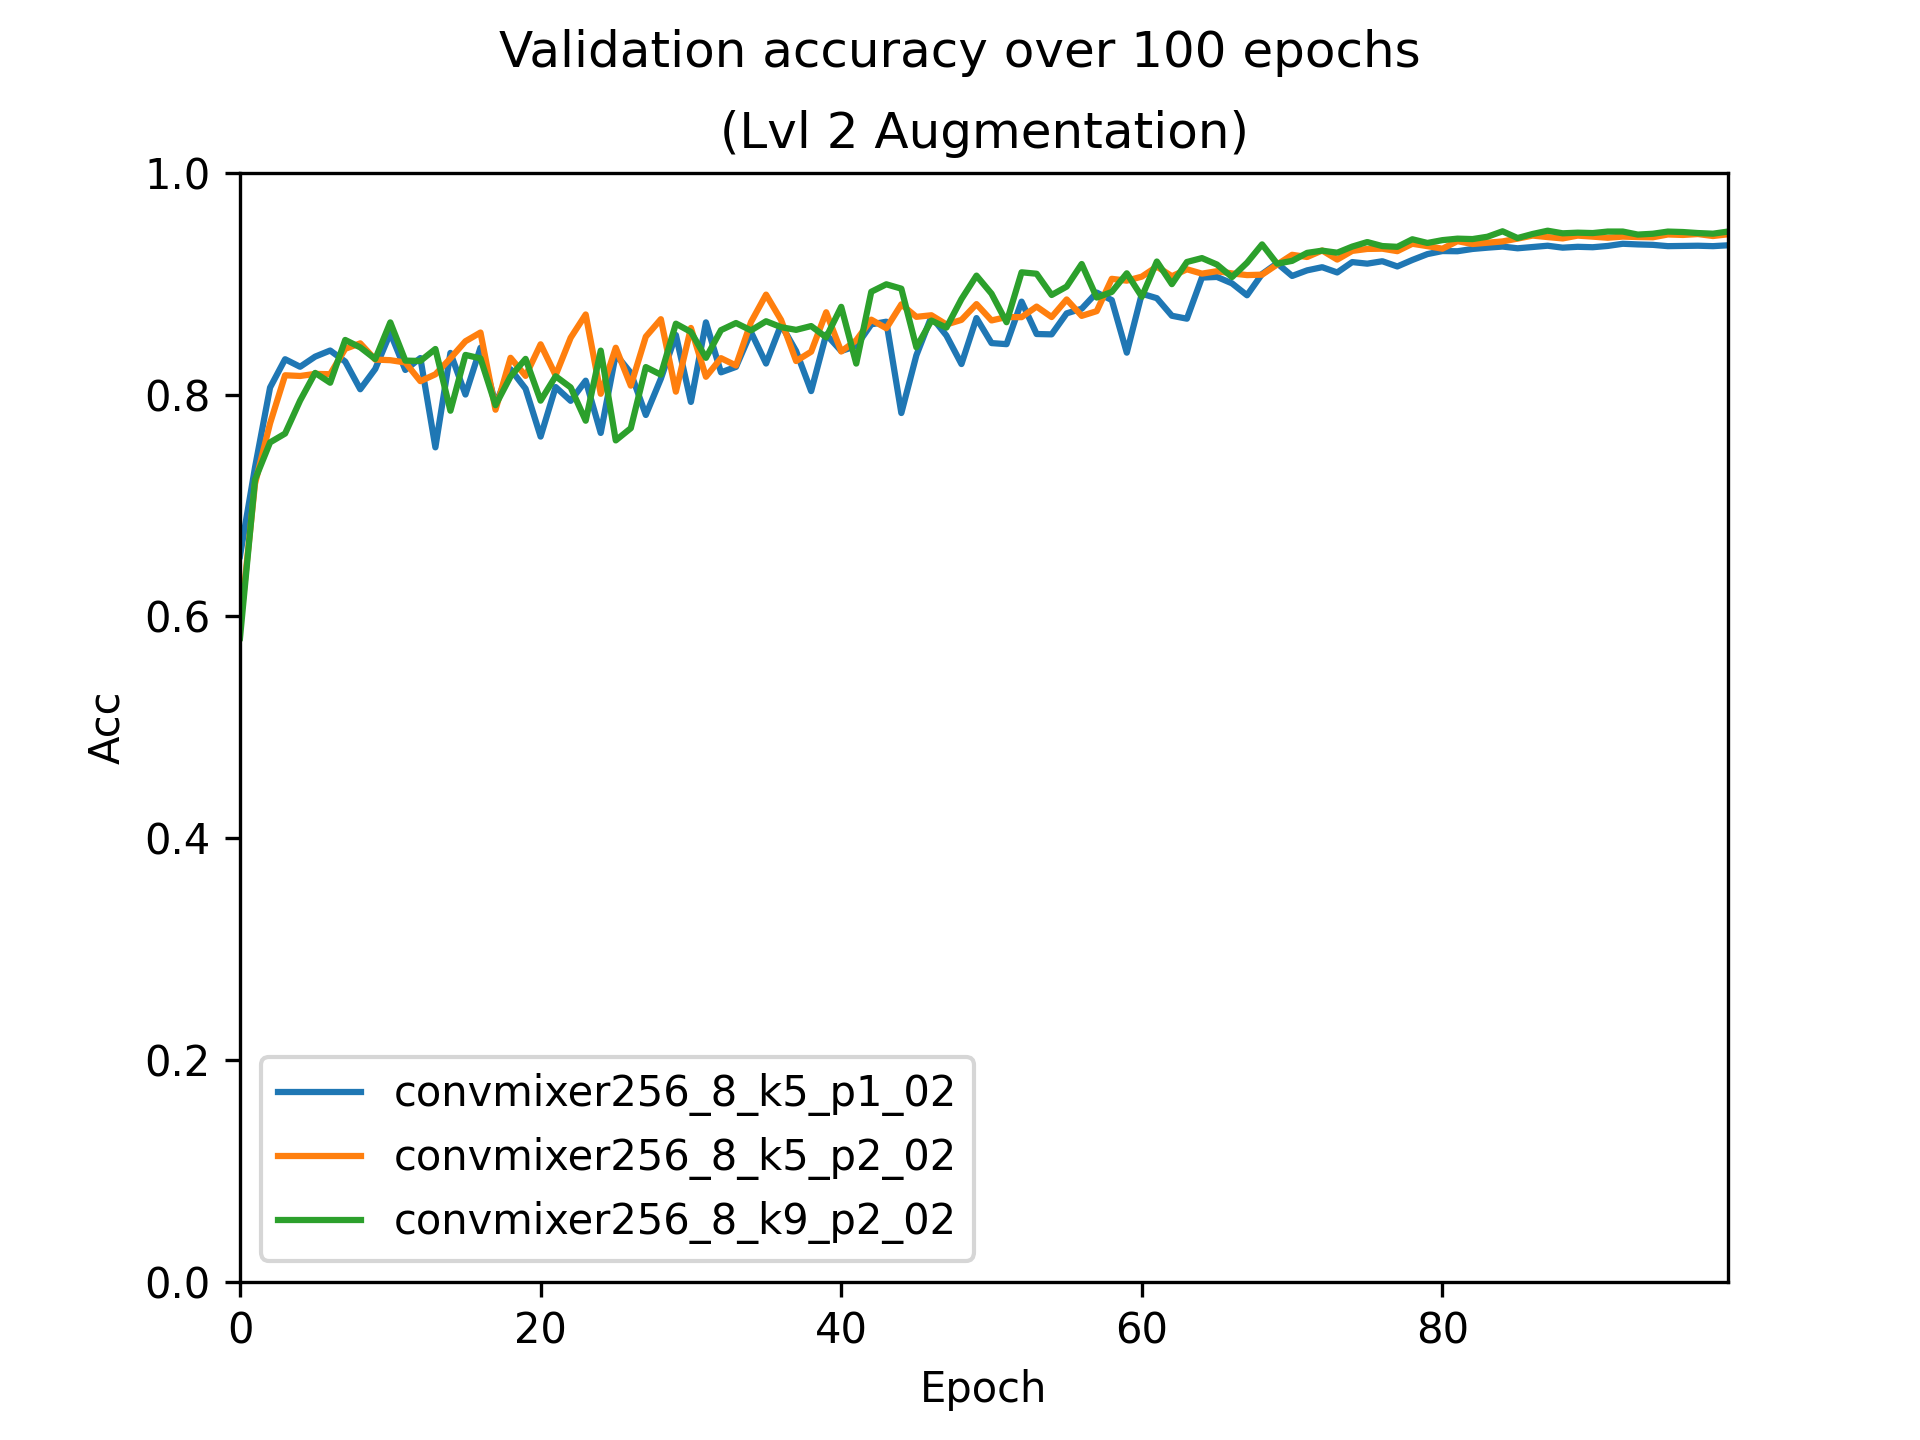
\includegraphics[width=\linewidth]{val_lvl2.png}
    \caption{Comparison of validation accuracy for ConvMixer256/8 with varying kernel and patch sizes at augmentation level 2.}
  \end{figure}

\todo{discuss experiment results}

\section{Results}

For our final results, we attempted to push the ConvMixer256/8(\verb|kernel_size=5, patch_size=2|) to 95\% accuracy. Our initial experiments indicated that a kernel size of 5 and patch size of 2 presented the best balance between model performance and training speed. We increased the number of training epochs and, to preempt the training saturation we observed previously, added CutMix regularization \citep{Yun2019} to the model, a method which had shown promise in shorter experiments we performed. Training for 200 epochs, the model achieved 95.0\% accuracy on the test data.


For a final comparison, we also trained a similarly sized ResNet based on the architecture described by \citet{He2015} for use with CIFAR-10. Our implementation, which we name ResNet/S-38 to distinguish it from the typical ResNet architectures, has 561,370 parameters. We applied the same regularization and trained the model for 200 epochs. The model achieved 94.7\%, essentially on par with our final ConvMixer model. It also had a significantly higher training throughput: 0.12 seconds per sample vs 0.17 seconds per sample for the ConvMixer.

\begin{figure}
    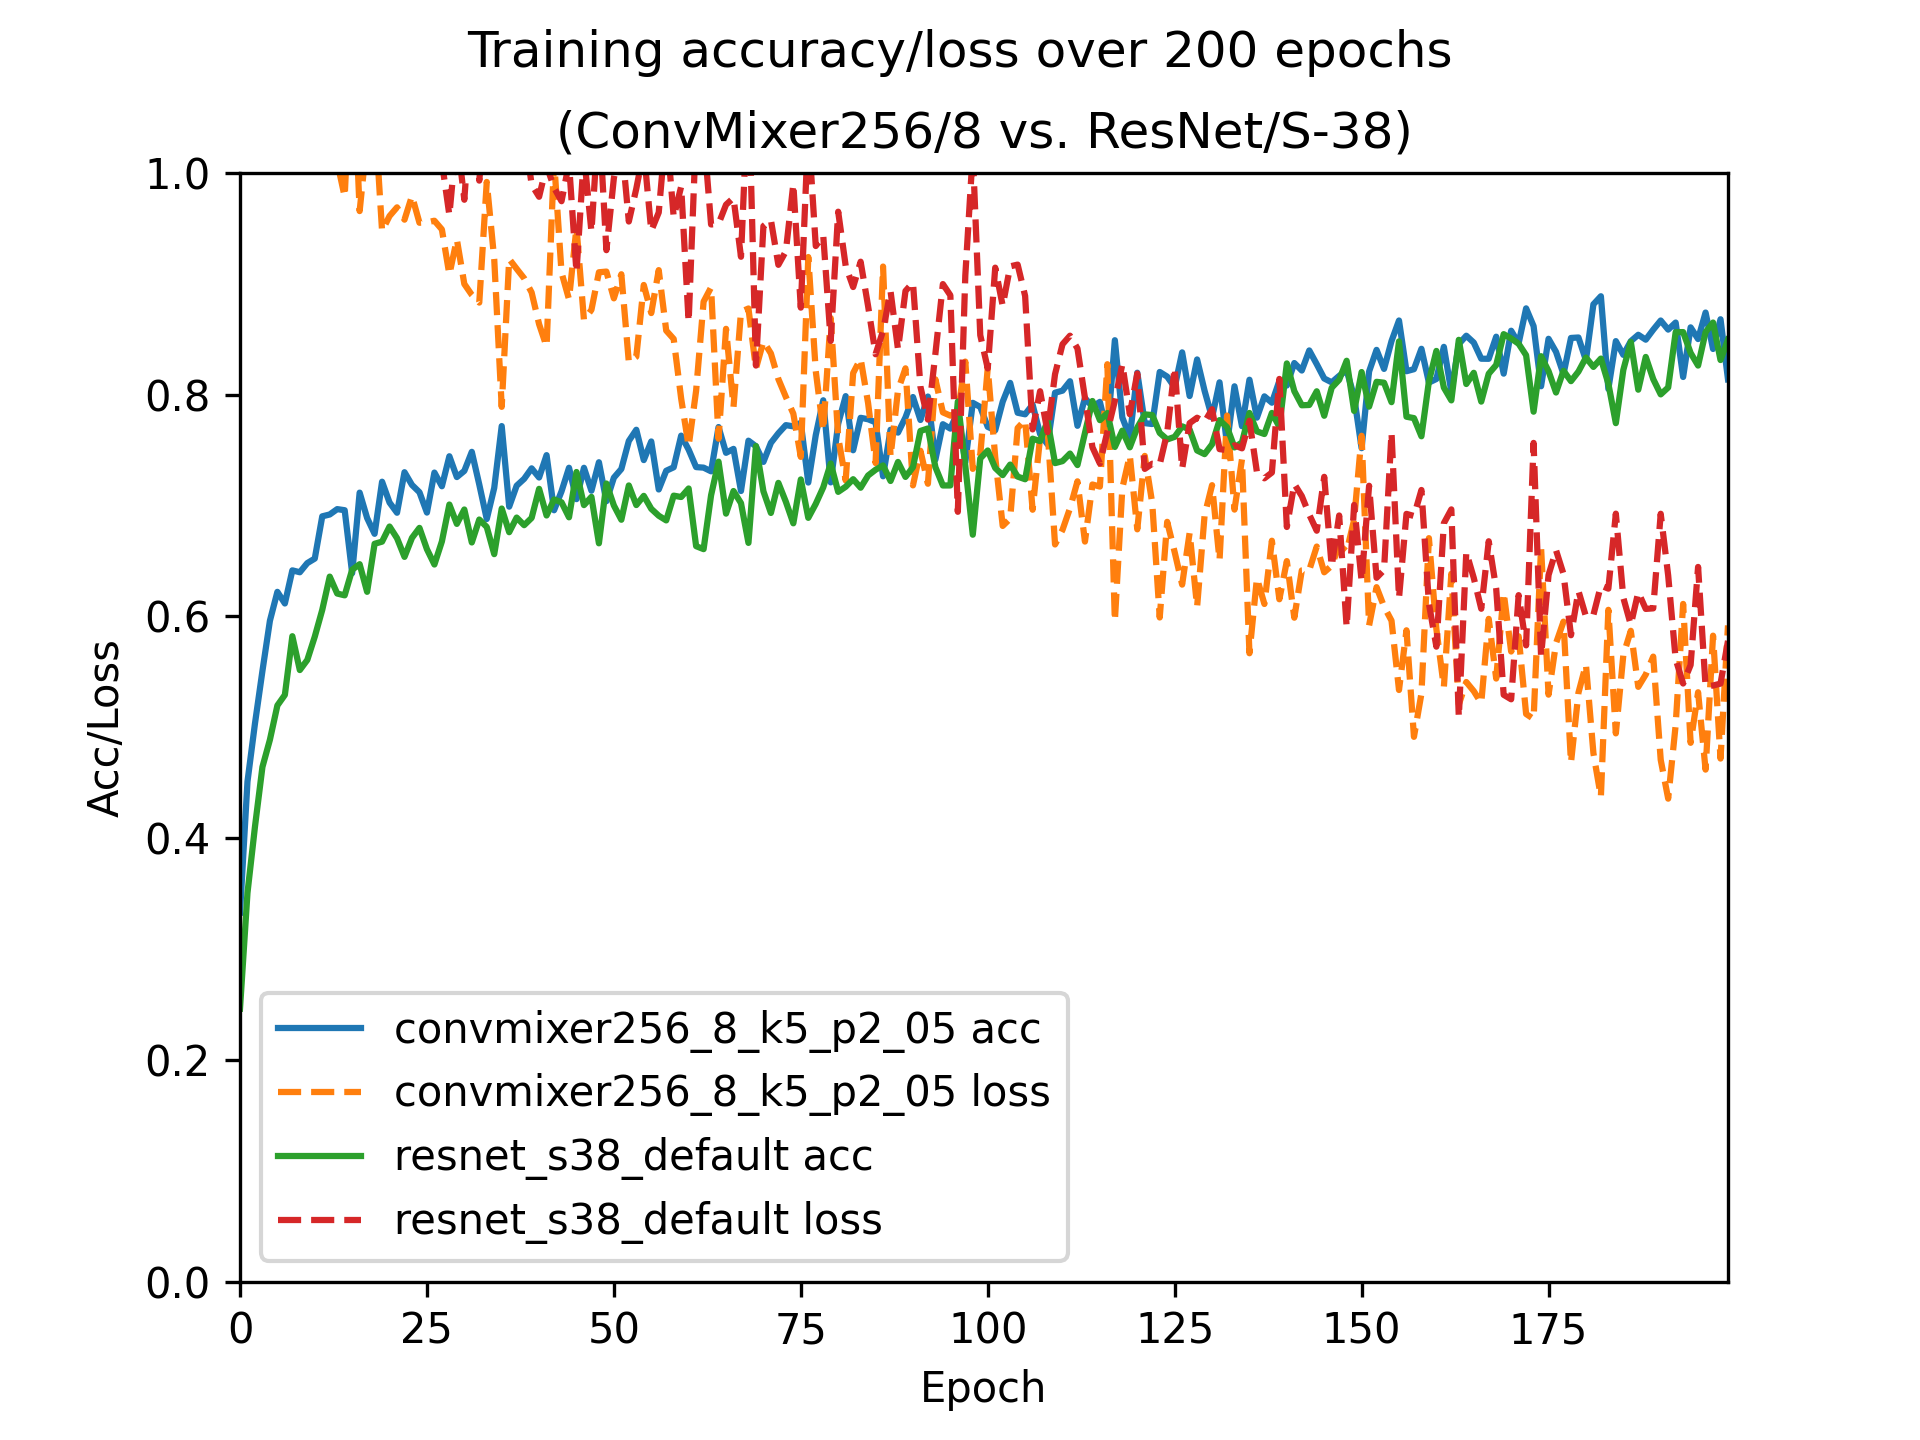
\includegraphics[width=\linewidth]{final_training.png}
    \caption{Comparison of model training metrics for ConvMixer256/8 (kernel size=5, patch size=2) and ResNet/S-38.}
  \end{figure}

  \begin{figure}
    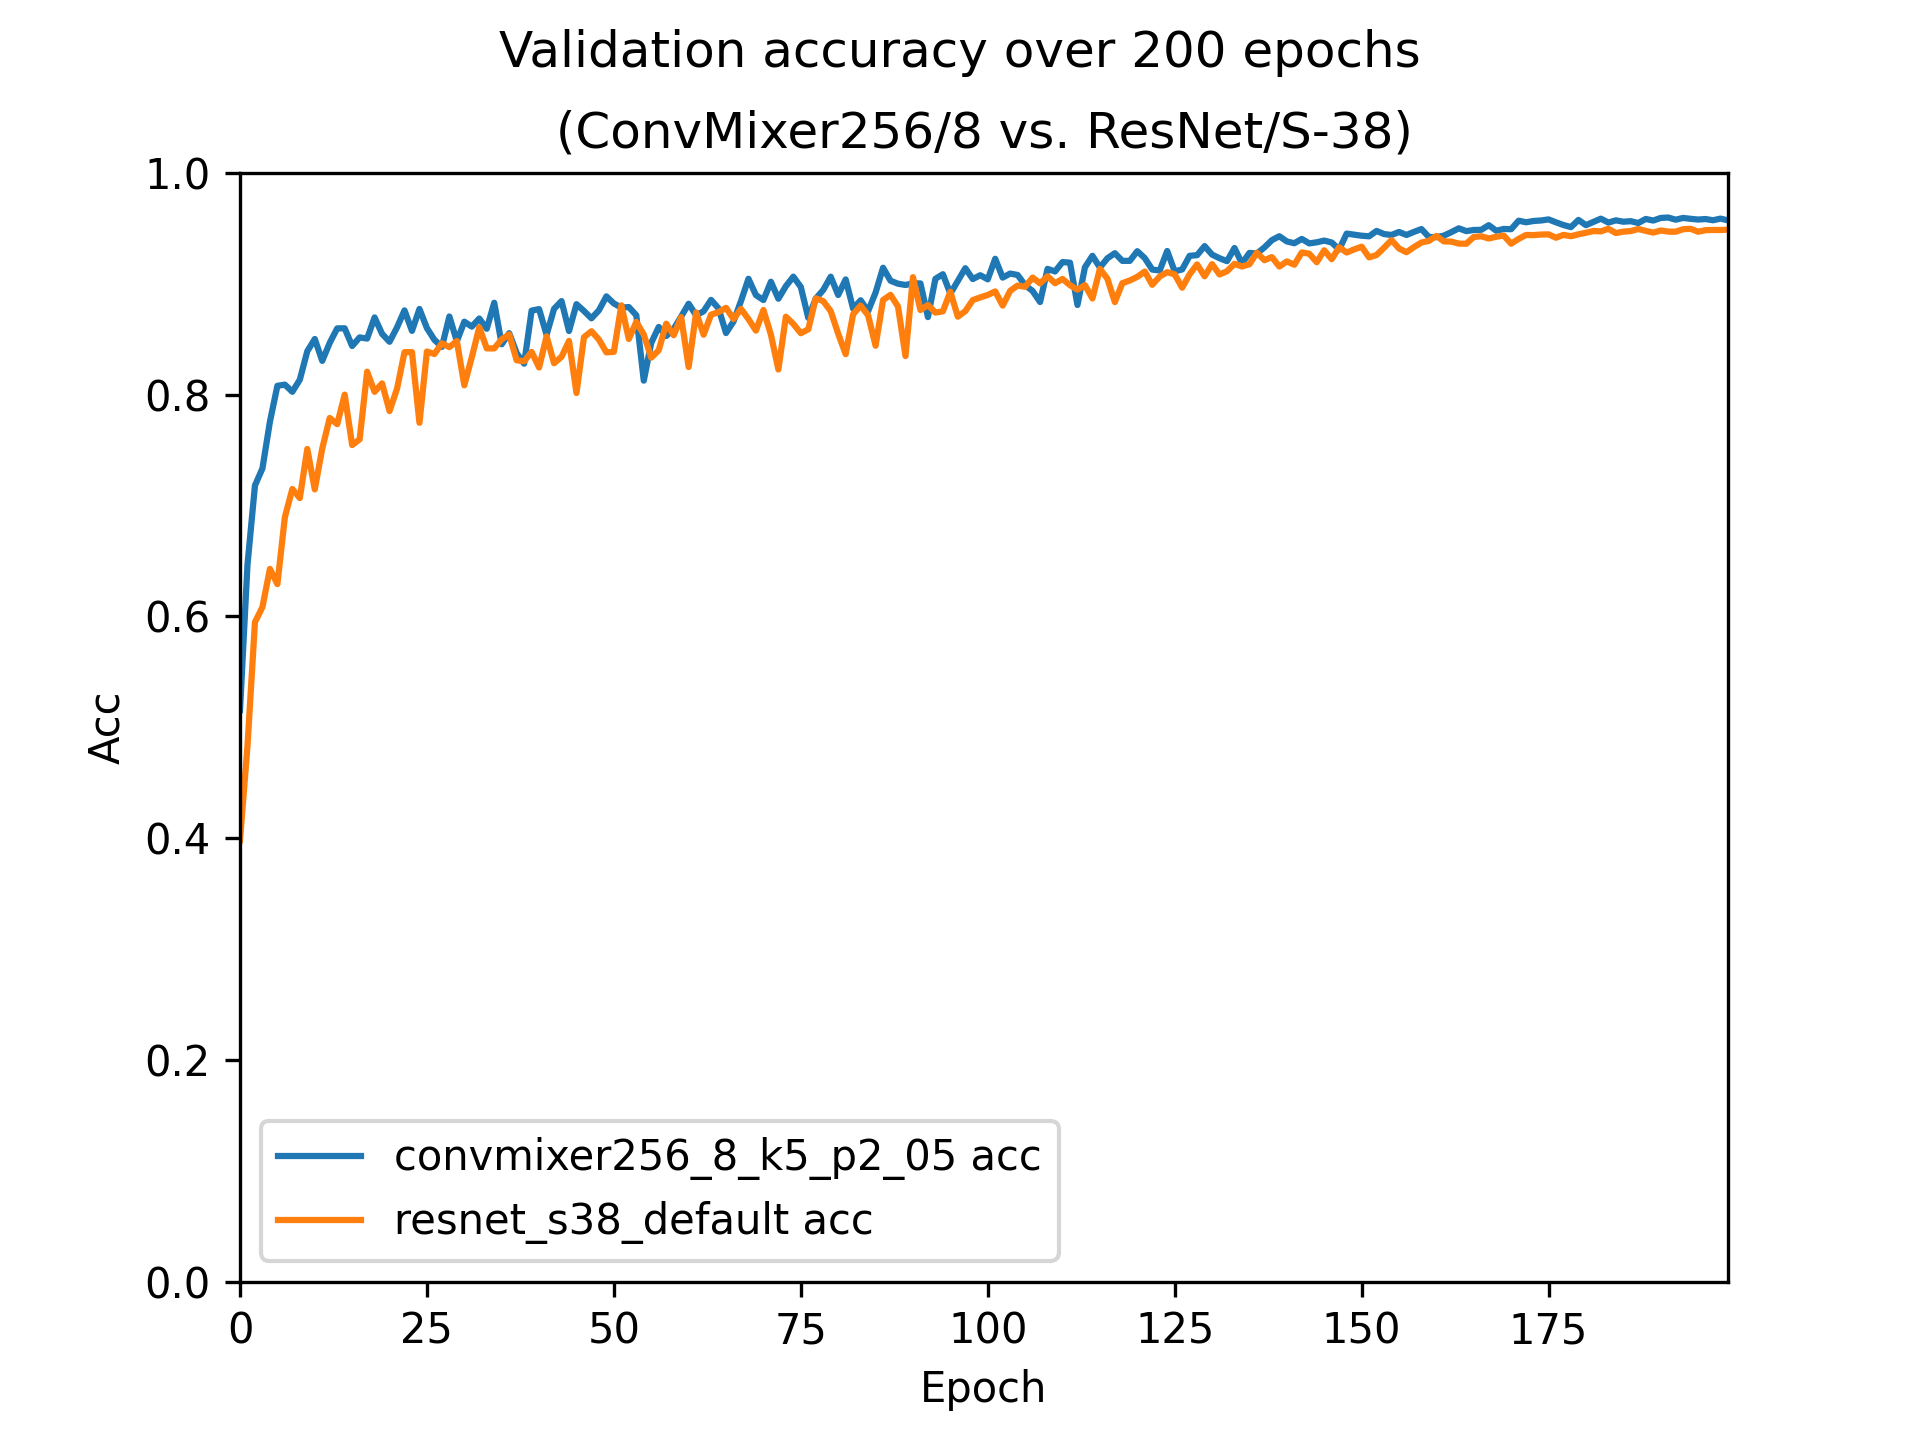
\includegraphics[width=\linewidth]{final_validation.png}
    \caption{Comparison of validation accuracy for ConvMixer256/8 (kernel size=5, patch size=2) and ResNet/S-38.}
  \end{figure}

\appendix

\bibliography{convmixer_project}

\end{document}